\documentclass[8pt]{extarticle}

% Packages
\usepackage[T1]{fontenc}
\usepackage[utf8]{inputenc}
\usepackage{geometry}
\usepackage[colorlinks=true, urlcolor=blue, pdfborder={0 0 0}]{hyperref}
\usepackage{multicol} 
\usepackage{xcolor}
\usepackage{listings} %for SQL snippets
\usepackage{pdflscape} % for landscape pages
\usepackage{enumitem} %for formatting of lists
\usepackage{graphicx} %for scaling tabular environments
\usepackage{tabularx} %for allowing wrapping columns whilst respecting rescaling.
\usepackage{tcolorbox} %for highlighted boxes

\usepackage{lipsum} %for sample paragraphs, delete at end

%correct handling of _ inside inline code snippet
\lstset{
    language=Python,
    basicstyle=\ttfamily,
    literate={_}{{\_}}1
}


% Page configuration
\geometry{a4paper, landscape, top=10mm, bottom=10mm, left=10mm, right=10mm, columnsep=10mm,}

% no indent globally
\setlength{\parindent}{0pt}

% Python snippet environment
\lstdefinestyle{python}{
    language=Python,
    basicstyle=\small\ttfamily,
    keywordstyle=\color{blue},
    commentstyle=\color{gray},
    stringstyle=\color{teal},
    identifierstyle=\color{black},
    numberstyle=\tiny\color{gray},
    keywordstyle=[2]\color{purple},
    keywordstyle=[3]\color{orange},
    breaklines=true,
    showstringspaces=false,
    tabsize=4,
    %numbers=left,
    numbersep=5pt
}

% Lined separator for headings
\newcommand{\heading}[1]{%
    \noindent
    \rule{\linewidth}{0.4pt}
    \begin{center}
        \vspace{-1ex}
        \textbf{#1}        
        \vspace{-2.5ex}
    \end{center}
    \rule{\linewidth}{0.4pt}
}


\begin{document}

% Remove page numbers for this page
\thispagestyle{empty} 

% Title
\begin{center}   
{\huge\textbf{Pandas Cheat Sheet}}\\
\vspace*{0.25cm}
More information can be found in the docs: \href{https://pandas.pydata.org/docs/reference/index.html}{https://pandas.pydata.org/docs/reference/index.html} \\
\hspace*{4.73cm} \href{https://matplotlib.org/stable/api/index.html}{https://matplotlib.org/stable/api/index.html}
\vspace*{0.05cm}
\end{center}

\begin{multicols}{4}
\setlength{\columnseprule}{1pt} % Add vertical line between columns


\heading{MOCK DATAFRAME AND SETUP}

Note that pandas, matplotlib and seaborn are not standard packages and need to be installed and imported. They are imported using common shorthand as follows:

\begin{lstlisting}[style=Python]
import pandas as pd
import matplotlib.pyplot as plt
import seaborn as sns
\end{lstlisting}
\vspace{0.5ex}

The running example in the cheat sheet will be a dataframe containing information about students. Later we will introduce a `exams' dataframe to perform joins etc. \\

Mock data: Our mock data contains information on five students, namely their `name', `DOB', `sex', `postcode' and whether they are a 
`current\_student' ($1$ if yes, $0$ if no).
\begin{lstlisting}[style=Python]
student_data = {
    "name": ["Alice", "Bob", "Charlie", "David", "Eva"],
    "DOB": ["2001-05-14", "2000-08-30", "2002-12-11", "1999-07-22", "2003-01-19"],
    "sex": ["F", "M", "M", "M", "F"],
    "postcode": ["AA345", "AB456", "AC567", "AB678", "AB789"],
    "current_student": [1, 0, 1, 0, 1]
}
\end{lstlisting}
\vspace{0.5ex}

Our mock dataframe (when we create it in the next section) will be called `students'.\\

\begin{tcolorbox}[width=\columnwidth, colback=white!95!black] 
For many objects/functions only some of the passable arguments will be discussed, the non-discussed ones will be replaced by `...' - see the documentation for a full description of all arguments.
\end{tcolorbox}

\heading{DATAFRAMES}

Dataframes are tables in pandas. They are a pandas object given as follows:

\begin{lstlisting}[style=Python]
class pd.DataFrame(data=None, index=None, ...)
\end{lstlisting}

\begin{enumerate}
    \item data: usually a dictionary, but can also be ndarrays, lists of dictionaries/Series etc.
    \item index: a list with index labels   
\end{enumerate}

Dataframes may also be obtained from `.csv' files or otherwise. This is done using 

\begin{lstlisting}[style=Python]
pd.read_csv(file_path, sep, index_col, names, ...)
\end{lstlisting}

\begin{enumerate}
    \item file\_path: A string containing the path to the file to be imported.
    \item sep: Specify the delimiter, this is `,' by default. Passing, for example, `|' allows .tsv files to be read in.
    \item index\_col: Specify column(s) to become the (multi)index
    \item names: Pass a list of column labels. To replace the current column laebel in the .csv pair the `columns' argument with the argument `header = 0'.
\end{enumerate}

Example:
\begin{lstlisting}[style=Python]
students = pd.DataFrame(student_data)
print(students)
\end{lstlisting}

Output:
\begin{center}
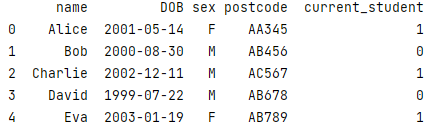
\includegraphics[scale = 0.5]{images/mock_df.png}
\end{center}

\heading{INSPECTING DATAFRAMES}

There are many methods and attributes on a DataFrame object wich we can use to obtain information about it. We use a DataFrame object called `df'.\\

\resizebox{\columnwidth}{!}{%
\begin{tabular}{|c|c|}
    \hline
     Method/attribute & Short description\\
     \hline
     df.columns & Index/list of column names\\ 
     \hline
     len(df) & number of rows\\
     \hline
     df.shape & tuple (\#rows, \#columns)\\
     \hline
     df.head(n=5) & displays first $`n'$ rows of dataframe\\
     \hline
     df.tail(n=5) & displays last $`n'$ rows of dataframe\\
     \hline
     df.info() & information about dataframe\\
     \hline
     df.dtypes & column names and their dtypes\\
     \hline
\end{tabular}}\\

\columnbreak

For example, \lstinline[style=Python]!students.info()! gives output
\begin{center}
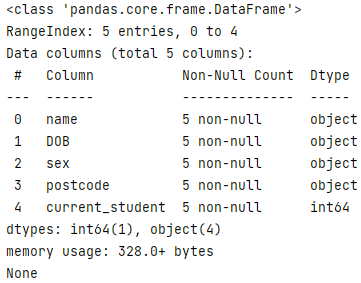
\includegraphics[scale = 0.6]{images/info()_method.png}
\end{center}
and \lstinline[style=Python]!students.dtypes! gives output
\begin{center}
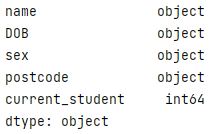
\includegraphics[scale = 0.6]{images/dtypes.png}
\end{center}
\heading{BASIC DATAFRAME ANALYSIS}

We can do basic analysis on dataframes, such as finding the minimum value in each column or finding the most common value in each column. We use a DataFrame object called `df'.\\

The methods in the following table return a Series object (see next section for a discussion on Series).\\

\resizebox{\columnwidth}{!}{%
\begin{tabular}{|p{0.45\columnwidth}|p{0.55\columnwidth}|}
    \hline
     Method & Short description\\
     \hline
     df.min() & finds the minimum value from each column\\ 
     \hline
     df.max() & finds the maximum value from each column\\
     \hline
     df.sum() & returns sums of the columns. For strings this is concatenation, for numeric columns is regular addition.\\
     \hline
     df.count() & counts non-NaN values in each column\\
     \hline
     df.mean(\newline numeric\_only=True) & finds mean of numeric columns\\
     \hline
     df.median(\newline numeric\_only=True) & finds median of numeric columns\\
     \hline
\end{tabular}}\\

The following two methods return DataFrame objects:\\


\resizebox{\columnwidth}{!}{%
\begin{tabular}{|p{0.45\columnwidth}|p{0.55\columnwidth}|}
    \hline
     Method & Short description\\
     \hline
     df.mode() & returns columns and their most common values\\ 
     \hline
     df.describe() & returns stats for each column such as mean, mode, median, percentiles. By default this is only for numeric columns, passing "include=`all' " produces descriptions for all columns.\\
     \hline
\end{tabular}}\\

E.g., students.describe(include=`all') gives...
\begin{center}
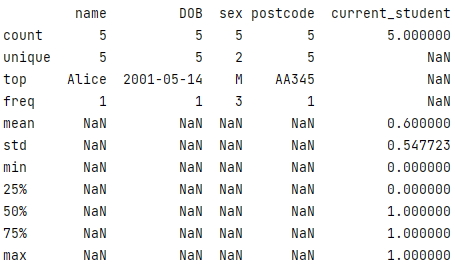
\includegraphics[scale = 0.5]{images/describe()_method.png}
\end{center}
\vspace{1ex}

\heading{SERIES \& SELECTING COLUMNS}

A series is a one-dimensional array with labels (roughly, it is an $n \times 1$ dataframe, but with slightly different behaviour). They are initialised using 

\begin{lstlisting}[style=Python]
pd.Series(data,index,...)
\end{lstlisting}

\begin{itemize}
\item Obtaining a Series as a column of a dataframe:

We can extract a column of a dataframe, df, as a Series as follows:
\begin{lstlisting}[style=Python]
df[column_name]
\end{lstlisting}
The index will be the index of the dataframe, the values will be the values in the column.

\item Selecting multiple columns of a dataframe:

To extract multiple columns of a dataframe we pass a list of column names, the resulting object will be a dataframe. 

\begin{lstlisting}[style=Python]
df[[col_name_1, col_name_2,...]]
\end{lstlisting}
\end{itemize}

\end{multicols}
\newpage
% Remove page numbers for this page
\thispagestyle{empty} 

\begin{multicols}{4}
\setlength{\columnseprule}{1pt} % Add vertical line between columns

\heading{BASIC SERIES ANALYSIS}

Methods such as sum, min, max work on Series too. They return a int/float/string object. A flowchart to keep in mind is:


\begin{center}
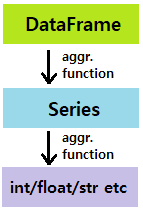
\includegraphics[scale = 0.65]{images/agg_functions_flowchart.png}
\end{center}

Some other methods and attributes of a Series, s, include:

\begin{itemize}
    \item s.values - returns values of the Series as an array
    \item s.index - gives information about the index/labels
    \item Have head(), tail(), info(), describe() etc.
    \item s.unique() - array containing distinct values in the series
    \item s.nunique() - number of distinct values
    \item s.nlargest(n=5) - returns the `n' largest values, by default `n=5'
    \item s.nsmallest(n=5) - ...
    \item s.value\_counts() - returns Series with labels given by values in the Series, s, and values given by number of occurrences.
\end{itemize}

For example, extracting the column `sex' from our dataframe `students' and printing value counts of the resulting Series can be done via:

\begin{lstlisting}[style=Python]
s = students['sex']
print(s.value_counts())
\end{lstlisting}

which gives output:

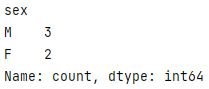
\includegraphics[scale = 0.6]{images/series_output.png}

\begin{tcolorbox}[width=\columnwidth, colback=white!95!black]
For dataframes we have \begin{lstlisting}[style=Python]
df.nlargest(n=5,columns)\end{lstlisting} where $n$ largest dataframe rows are returned based on values in the provided list of columns, `columns'. 
\end{tcolorbox}


\heading{INDEXING AND SORTING}

To set the index (or labels) of a dataframe using a list of values or an existing column we use

\begin{lstlisting}[style=Python]
df.set_index(keys,inplace = False)
\end{lstlisting}
where `keys' is either an array (of the correct length) or a column name.

\begin{tcolorbox}[width=\columnwidth, colback=white!95!black]
inplace - this optional argument replaces `df' with the modified dataframe if set to True, and returns a new dataframe if set to False. 
\end{tcolorbox}

To sort rows by values in given column(s) we use

\begin{lstlisting}[style=Python]
df.sort_values(by, ascending=True, inplace=False,key = None,...)
\end{lstlisting}
where `by' is a column name or list of column names to sort by. Whether to sort in ascending or descending order is decided using the optional argument `ascending'.\\

The argument `key' allows us to pass a (vectorised) function which is applied to the sorting column before sorting. 

For example, to sort our dataframe by length of the students name we use

\begin{lstlisting}[style=Python]
students.sort_values('name', key = lambda x: x.str.len())
\end{lstlisting}

which returns the dataframe

\begin{center}
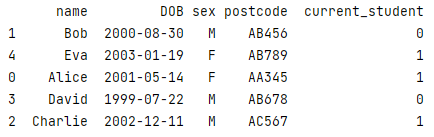
\includegraphics[scale = 0.53]{images/sorted_df.png}
\end{center}

To sort by index we can use 

\begin{lstlisting}[style=Python]
df.sort_index(ascending = True, inplace = False, ...)
\end{lstlisting}

\begin{tcolorbox}[width=\columnwidth, colback=white!95!black]
Both of these sorts work for Series too, but of course there is no column name to pass to the `sort\_values` method.
\end{tcolorbox}

\heading{ACCESSING ROWS}

To access rows of a dataframe or Series, we use `loc'. To  retrieve row(s) of a dataframe based on index name(s) we use

\begin{lstlisting}[style=Python]
df.loc[index_names]
\end{lstlisting}
where index\_names is either a single index name or a list of index names. This returns either a Series (if a single index name is passed) or a slice of the dataframe (if a list is passed).

\begin{tcolorbox}[width=\columnwidth, colback=white!95!black]
We can also pass slices, boolean arrays (of the correct length), boolean Series to loc. There is lots of flexibility, see the docs for more. 
\end{tcolorbox}

We can also extract the $n^{th}$ row using `.iloc', e.g. to extract the $5^{th}$ row of a dataframe, df, we use 
\begin{lstlisting}[style=Python]
df.iloc[4] #indexing starts from 0.
\end{lstlisting}

\begin{tcolorbox}[width=\columnwidth, colback=white!95!black]
Additionally, we can pass a second list consisting of column names, so we do not have to extract all columns for the specified rows. 
\end{tcolorbox}

\heading{FILTERING DATAFRAMES}

We can create a boolean series (a Series consisting of True/False values) by applying a comparison operator to a Series. For example

\begin{itemize}
    \item equals (==): \\
    e.g. \lstinline[style=Python]!df[column_name] == some_value !
    \item not equal (!=)
    \item less, greater, leq, geq (<, >, <=, >=)
    \item \lstinline[style=Python]!.between(left,right)! (inclusive by default): \\
    e.g. \lstinline[style=Python]!df[column_name].between(5,10) !
    \item \lstinline[style=Python]!.isin(value: list-like)!: \\
    e.g. \lstinline[style=Python]!df[column_name].isin(lst_of_values) !
    \item \lstinline[style=Python]!.isna(), .notna()! (check if values are null, not null): e.g. \lstinline[style=Python]!df[column_name].isna() !
\end{itemize}

This can also be referred to as a (boolean) mask. If boolean\_series is our mask then we extract the rows evaluating to True using
\begin{lstlisting}[style=Python]
df[boolean_series]
\end{lstlisting}

\begin{tcolorbox}[width=\columnwidth, colback=white!95!black]
This has the same behavior as 
\begin{lstlisting}[style=Python]
df.loc[boolean_series].
\end{lstlisting}
To extract columns based on Trues within a boolean list (boolean\_list) we use 
\begin{lstlisting}[style=Python]
df.loc[:,boolean_list].
\end{lstlisting}
The `:' means `select all rows' and boolean\_list is now targeting columns (since it is the second argument in loc).
\end{tcolorbox}

We can also extract rows using a boolean list (ensuring the list is of the correct length i.e., the same length as the number of rows).\\

We combine conditions using AND (\&) or OR (|). Boolean Series are negated using tilde ($\sim$). \\

For example, to print rows containing females who are current students from our `students' dataframe, we use:

\begin{lstlisting}[style=Python]
mask = (students['sex'] == 'F') & (students['current_student'] == 1)
print(students[mask])
\end{lstlisting}
Output:

\begin{center}
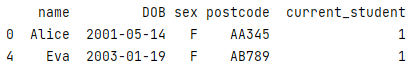
\includegraphics[scale = 0.53]{images/filtered_output.png}
\end{center}

\heading{ADDING AND REMOVING DATA}

To add a column called `new\_column\_name' to a dataframe we use 
\begin{lstlisting}[style=Python]
df['new_column_name'] = values
\end{lstlisting}
where values could be a constant, a list-like object, a dict, a Series etc. \\
In particular, we could create new columns using functions on old ones (including basic arithmetic/string functions). \\
e.g. \lstinline[style=Python]!df[new_doubled_column] = df[old_column]*2 !  \\

To remove rows or columns we use 
\begin{lstlisting}[style=Python]
df.drop(index=None, columns=None, inplace=False,...)
\end{lstlisting}
where `index' is a list of index names to be dropped, and `columns' is a list of column names to be dropped.

\end{multicols}
\newpage
% Remove page numbers for this page
\thispagestyle{empty} 

\begin{multicols}{4}
\setlength{\columnseprule}{1pt} % Add vertical line between columns

\heading{UPDATING VALUES}

Firstly, we can update a value if we know its exact location:
\begin{lstlisting}[style=Python]
df.loc[its_index,its_column] = new_value
\end{lstlisting}
To replace dynamically we can use the replace method:
\begin{lstlisting}[style=Python]
df[column_name].replace(to_replace=None, value=None, inplace=False,...)
\end{lstlisting}
where `to\_replace' should be a value/list of values/regex expression etc, and `value', gives the replacement(s). \\
Alternatively, `to\_replace' can be a dict object, then `value' should be left blank.\\

To rename indices or column headers we use:
\begin{lstlisting}[style=Python]
df.rename(index=None, columns=None, inplace=False,...)
\end{lstlisting}
where `index' and/or `columns' should be a mapper (such as a dict object) or a function.

\heading{DATATYPES}

The catchall dataype is `object'. It takes up lots of space. The (Series) method 
\begin{lstlisting}[style=Python]
.astype() 
\end{lstlisting}
can be used to convert the type of a column of a dataframe.
There is no `inplace' here, so to update the datatype we need to do:
\begin{lstlisting}[style=Python]
df[column_name] = df[column_name].astype(dtype)
\end{lstlisting}
Examples of dtypes include:
\begin{itemize}
    \item int, float
    \item bool
    \item string
    \item datetime, timedelta
    \item category (this is good for columns with specific set of values it can take e.g. \lstinline[style=Python]![0,1] ! for the current\_student column for our `students' dateframe.
\end{itemize}

There also exists a pandas method to convert values to numeric datatypes,
\begin{lstlisting}[style=Python]
pd.to_numeric(arg,errors,...)
\end{lstlisting}The argument can be a scalar, list-like, Series (e.g. a dataframe column). `errors' tells pandas how to deal with values which cannot be converted, either `raise' or `coerce'.

\heading{WORKING WITH NULL VALUES}

We briefly discuss three methods to deal with null values. 
\begin{itemize}
    \item \lstinline[style=Python]! .isna() ! - a method on Series and Dataframes. Returns a Series or Dataframe with True if null and False otherwise.
    \item \lstinline[style=Python]!.dropna() ! - for Series, creates a new Series with null values removed. For Dataframes it removes rows with at least one null value, but parameters can customise its behavior. See docs.
    \item \lstinline[style=Python]!.fillna(value, inplace,...) ! - fills null values with a given value, also a mapper can be passed. See docs.
\end{itemize}

\heading{DATES AND TIMES}

To convert columns to a date or time we can use the pandas method 
\begin{lstlisting}[style=Python]
pd.to_datetime(arg,dayfirst=False, yearfirst=False, format = None,...)
\end{lstlisting}
The argument `arg' can be str, list, Series, etc. The method automatically parses a lot of datatime formats. However, can specify dayfirst, yearfirst or pass a format e.g. \lstinline[style=Python]!"%d/%b/%y"!. Search "Python date format codes" or similar for info on this.\\

To parse a column of a dataframe we use 

\begin{lstlisting}[style=Python]
df[column_name] = pd.to_datetime(df[column_name])
\end{lstlisting}

We access properties of datetime objects using .dt. Some examples are:
\begin{itemize}
    \item \lstinline[style=Python]!.dt.{year,month,hour,day,minute,second}! - extracts year,month,...,second from the datetime object.
    \item \lstinline[style=Python]!.dt.dayofweek! - (Monday = 0,Sunday = 6).
    \item \lstinline[style=Python]!.dt.month_name()!
\end{itemize}

We can do comparisons using datetimes and their properties.\\ We can add and subtract datetimes, which result in timedelta objects. Properties of timedelta objects are obtained using \lstinline[style=Python]!.dt.!.\\

\heading{GROUPING}

We can group rows in the table based on the values in given columns via
\begin{lstlisting}[style=Python]
df.groupby(by = None,...)
\end{lstlisting}
where `by' should be a column name or a list of column names. \\Additionally, one can pass a function applied to a column. e.g. if grouping by the first letter of a name we can pass \lstinline[style=Python]!df.['name'].str[0]! directly to the \lstinline[style=Python]!.groupby()! method.\\

This returns a pd.Dataframe.groupby object (let `gbo' be an arbitrary such object).\\

Some methods and attributes of groupby objects:

\begin{itemize}
    \item \lstinline[style=Python]!gbo.ngroups! - returns the number of groups.
    \item \lstinline[style=Python]!gbo.groups! - returns dictionary with groups and indices within each group.
    \item \lstinline[style=Python]!gbo.first()! - returns dataframe (with the grouped column as index) with the first row from each group.
    \item \lstinline[style=Python]!gbo.get_group(name)! - returns the rows (as a dataframe) in the group with the given name.
\end{itemize}

For example, the code
\begin{lstlisting}[style=Python]
gbo = students.groupby('sex')
print(gbo.ngroups)
print(gbo.groups)
\end{lstlisting}

gives output 

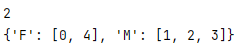
\includegraphics[scale = 0.7]{images/grouping_eg.png}

\begin{tcolorbox}[width=\columnwidth, colback=white!95!black]
It is possible to iterate over a gbo:
\begin{lstlisting}[style=Python]
for group_name, group_rows in gbo:
    #do something
\end{lstlisting}
where \lstinline[style=Python]!group_rows! has value \lstinline[style=Python]!gbo.get_group(group_name)!.
\end{tcolorbox}

There are methods we can apply to groupby objects. We can apply them to grouped dataframe (e.g. \lstinline[style=Python]! df.groupby(group_column)!) or select a specific column first and apply function to the grouped Series (i.e. \lstinline[style=Python]!df.groupby(group_column)[column_name]!):

\begin{itemize}
    \item \lstinline[style=Python]!gbo.size()! - returns Series with the size of each group (this includes NaN values).
    \item \lstinline[style=Python]!gbo.count()! - counts number of non-NaN values in each column from each group.
    \item \lstinline[style=Python]!gbo.describe()! - gives some statistics of numerical columns for each group.
    \item \lstinline[style=Python]!gbo.mean()!, \lstinline[style=Python]!gbo.median()! - should pass `numeric\_only=True' to both the mean and median methods.
\end{itemize}

The method \lstinline[style=Python]! .agg(func)! can be used to apply more complicated functions, or apply different functions to different columns.

\begin{itemize}
    \item \lstinline[style=Python]! gbo.agg('min')! - same as \lstinline[style=Python]!gbo.min()!.
    \item \lstinline[style=Python]! gbo.agg(['min','max'])! - applies min and max to all (numeric) columns.
    \item Alternatively, can pass dictionary to apply different functions to different columns \\
    e.g. \lstinline[style=Python]! gbo.agg({column_1: "mean", column2: "min"})!
    \item can pass custom functions too, these functions should accept a Series/dataframe as the argument
    \item To name the resulting columns we use `\lstinline[style=Python]!pd.NamedAgg!' e.g.\\
    \lstinline[style=Python]!gbo.agg(named_column = pd.NamedAgg(column_name,func))!
\end{itemize}

For example, the code
\begin{lstlisting}[style=Python]
gbo = students.groupby('sex')
print(gbo.agg({'name': 'min','current_student': ['mean','median']}))
\end{lstlisting}

gives output 

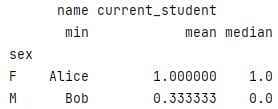
\includegraphics[scale = 0.65]{images/agg_functions.png}

In the above example we have two layers of column labels, namely level $0$ for the original column name, and level $1$ for the name of the function being applied. This is known as hierarchical labelling. 

\end{multicols}
\newpage
% Remove page numbers for this page
\thispagestyle{empty} 
\begin{multicols}{4}
\setlength{\columnseprule}{1pt} % Add vertical line between columns

\heading{HIERARCHICAL INDEXING}

Hierarchical (or multi-level) indexing can occur if dataframe is grouped by multiple columns. For example:
\begin{lstlisting}[style=Python]
df.set_index([column_name,another_column_name], inplace=True)
\end{lstlisting}
Here, \lstinline[style=Python]!df.index! returns \lstinline[style=Python]!MultiIndex! (indices are tuples).

Sorting rows using multi-level indices is done as follows:
\begin{itemize}
    \item \lstinline[style=Python]!df.sort_index(level=None)! - passing \lstinline[style=Python]!level=n! sorts by the index at level $n$.
    \item \lstinline[style=Python]!df.sort_index(level,ascending)! - can pass list of levels and `ascending' list (of same length) of True/Falses.
\end{itemize}

Can access rows using `.loc[$\,$]' as follows:
\begin{itemize}
    \item \lstinline[style=Python]!df.loc[level_0_index_value]! - access rows using the level $0$ index.
    \item \lstinline[style=Python]!df.loc[tuple_of_values]! - access rows using index tuple 
    \item \lstinline[style=Python]!df.loc[:,level_1_index_value,:]! - access by the level $1$ index, etc.
    \item The cross section method, \lstinline[style=Python]!.xs(..)!, exists for more cumbersome accessing (i.e. if there are many levels).
\end{itemize}

\begin{tcolorbox}[width=\columnwidth, colback=white!95!black]
Using group by and aggregate functions can produce hierarchical columns. These are accessed using tuples, e.g. \\
\lstinline[style=Python]! df[('level_0_heading', 'level_1_heading')]!.
\end{tcolorbox}

We can strip and produce multi-level indices using stack/unstack:
\begin{itemize}
    \item unstack - used to convert level of multi-index to a column e.g. \lstinline[style=Python]!df.unstack(level=n)!
    \item \lstinline[style=Python]!df.stack()! - convert $(m \times n)$ dataframe to a $(m \times n,1)$ dataframe by converting columns into multi-index.
\end{itemize}


To group by indices of a certain level we use 

\begin{lstlisting}[style=Python]
df.groupby(level=n)
\end{lstlisting}

Can also pass a list of levels to `level', or alternatively can pass index names.

\columnbreak

\heading{WORKING WITH STRINGS}

Recall that we can convert textual columns from `object' type to `string' type via 

\begin{lstlisting}[style=Python]
df[column_name] = df[column_name].astype("string")
\end{lstlisting}

For this section let $`s'$ be a Series object with textual values (either type object or string, it doesn't matter), for example, a column of a dataframe.

To apply string methods to a Series, s, apply them using \lstinline[style=Python]!s.str.!\\

Some examples are:

\begin{itemize}
    \item \lstinline[style=Python]!s.str.upper()! - all caps 
    \item \lstinline[style=Python]!s.str.lower()! - all lower case
    \item \lstinline[style=Python]!s.str[n]! - the $n^{th}$ character of each string 
    \item \lstinline[style=Python]!s.str.strip(to_strip = None)! - strips leading and trailing whitespace by default, if string of characters passed using `to\_strip' then these are striped instead. There also exists lstrip, rstrip.
    \item \lstinline[style=Python]!s.str.split(pat=None, expand=False)! - splits on spaces (or passed characters `pat'). This method produces Series where values are lists. If `expand=True' then it creates a dataframe by expanding the splitting lists.
    \item \lstinline[style=Python]!s.str.replace(to_replace, value)! - `to\_replace' and `value' can be str, regex, list of strings, dict (if dict then `value' shouldn't be provided) among others.
\end{itemize}

For example, suppose we wished to count the number of students (past and present) from each postcode area (i.e. `AA', `AB' or `AC'). To do so we can apply a string function to the postcode, then group, then find the size. 

\begin{lstlisting}[style=Python]
gbo = students.groupby(students['postcode'].str[:2])
print(gbo.size())
\end{lstlisting}

with output

\begin{center}
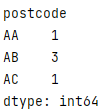
\includegraphics[scale = 0.65]{images/group_by_postcode_area.png}    
\end{center}

\columnbreak

\heading{APPLY, MAP, APPLYMAP}

To apply a (non-vectorised) function to a Series we use the pandas.Series method
\begin{lstlisting}[style=Python]
pd.Series.apply(func,arg=()).
\end{lstlisting}
If the function needs additio.nal arguments, these should be passed using `arg'. This returns a new Series with values given by the function applied (elementwise/rowwise) to the original values.\\

We can also apply maps to Series using
\begin{lstlisting}[style=Python]
pd.Series.map(arg)
\end{lstlisting}
For example, given Series, s, with values $1,2,3$ and wishing to change to $1^{st}$, $2^{nd}$, $3^{rd}$ can be done using
\begin{lstlisting}[style=Python]
s.map({1:'1st',2:'2nd',3:'3rd'})
\end{lstlisting}

To apply a function elementwise to every value in a dataframe (and return a new dataframe) we use
\begin{lstlisting}[style=Python]
df.applymap(func)
\end{lstlisting}

\heading{JOINING SERIES \& DATAFRAMES}

To join series together we use the pandas' concat method:
\begin{lstlisting}[style=Python]
pd.concat(objs,axis,join,ignore_index)
\end{lstlisting}
where `objs' should be a list of Series, `axis = 0' means stack vertically and `axis =1' means stack horizionally (i.e. join by index). Passing `ignore\_index=True' creates a new index for the combined Series. When joining series by index (i.e. `axis =1') pandas inserts NaN if a passed Series doesn't have a  particular index. This is an outer join (the default). To include only rows where all series have the index pass `join="inner"'.\\

As concat as a pandas method, concatenating dataframes works in much the same way. (Still have objs, axis, join that we can pass).\\

The last join to discuss is `merge'. This is an SQL-like join method, where we join on specific columns:

\begin{lstlisting}[style=Python]
df.merge(right,how,on,...)
\end{lstlisting}
where `right' is another dataframe, `how' is the join type, that is, `how' is one of left, right, outer, inner, cross. `on' is a column name or list of column names to join on.\\

\begin{center}
\underline{Examples of merges.}  
\end{center}

Let `exams' be another dataframe as follows:

\begin{center}
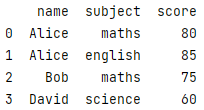
\includegraphics[scale = 0.6]{images/exams_df.png}
\end{center}

An inner join of `students' and `exams' is done as follows

\begin{lstlisting}[style=Python]
print(students.merge(exams,'inner','name'))
\end{lstlisting}

with output
\begin{center}
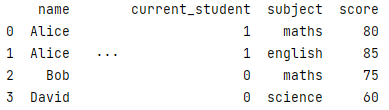
\includegraphics[scale = 0.5]{images/inner_merge.png}
\end{center}

Note that both `Charlie' and `Eva' are missing, as they had no exam scores. If we want them to be included we can use an outer join:

\begin{lstlisting}[style=Python]
print(students.merge(exams,'outer','name'))
\end{lstlisting}

with output
\begin{center}
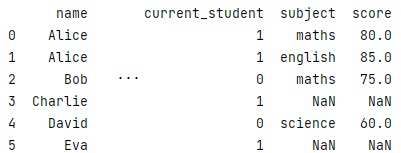
\includegraphics[scale = 0.5]{images/outer_merge.png}
\end{center}

Roughly, the different types of merges can be compared to different operations on two sets $A$ and $B$:

\begin{itemize}
    \item left - corresponds to $A$. i.e. all of $A$ is included, and elements of $B$ which happen to be in the intersection are also included, elements in $B \backslash A$ are discarded.
    \item right - corresponds to $B$. Analogous to above with roles of $A$ and $B$ switched.
    \item inner - like the intersection $A \cap B$
    \item outer - like the union $A \cup B$
    \item cross - like the cartesian product $A \times B$.
\end{itemize}
In our example above, the exams.name column (the set $B$) is a proper subset of the students.name column ( the set $A$). Therefore, `left' and `outer' will behave the same, and `right' and `inner' will behave the same.

\end{multicols}
\newpage
% Remove page numbers for this page
\thispagestyle{empty} 
\begin{multicols}{4}
\setlength{\columnseprule}{1pt} % Add vertical line between columns

\heading{MATPLOTLIB.PYPLOT}

All plotting functionality in pandas uses matplotlib behind the scenes, so it's useful to know some matplotlib (specifically matplotlib.pyplot). It's imported as follows

\begin{lstlisting}[style=Python]
import matplotlib.pyplot as plt
\end{lstlisting}

The first method to look at is 
\begin{lstlisting}[style=Python]
plt.plot()
\end{lstlisting}
This produces an empty plot as is. can pass lists, Series, two lists (first is x-axis, second is y-axis) and many kwargs such as:
\begin{itemize}
    \item color: e.g. `red', `blue', `\#[hex]', or any ccs recognised colour.
    \item linewidth: float
    \item linestyle: e.g. `-', `- -', `-.'. `dashed' ,`dotted'
    \item marker - marks the plotted line with a mark, e.g. `<', `>', `$\ast$'.
    \item label: a label for the plot
\end{itemize}

Using \lstinline[style=Python]!plt.plot(...)! will not display anything, to do this we must use 
\begin{lstlisting}[style=Python]
plt.show()
\end{lstlisting}
which displays all active figures.

\begin{tcolorbox}[width=\columnwidth, colback=white!95!black]
Tip: Within numpy we have the arange() method which can produce evenly spaced values within an interval. This is good for producing x-values for a function, for example.
\end{tcolorbox}

\underline{Figures, axes and plots.}\\

In matplotlib, a `plot' (the lines on a graph) lives on an `axis'. These axes in turn are placed in a `figure'. A diagram showing this is as follows:

\begin{center}
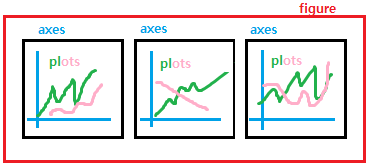
\includegraphics[scale = 0.64]{images/pyplot_levels.png}
\end{center}

So when we type \lstinline[style=Python]!plt.plot(...)! matplotlib implicity creates a figure and an axes for us.
\begin{lstlisting}[style=Python]
plt.plot(...)
plt.plot(...)
plt.show()
\end{lstlisting}
This code creates two plots on the same (implicitly created) axis contained in a (implicated created) figure. Whereas the code
\begin{lstlisting}[style=Python]
plt.plot(...)
plt.figure(figsize=None, dpi=None,...)
plt.plot(...)
plt.show()
\end{lstlisting}
places the first plot on the first axis in the first figure (all implicit), with the second plot being placed on a new (implicitly created) axes within the newly created figure. 

We may pass a `figsize' and a `dpi' to change the size of the figure. There are many other arguments to customise it, such as creating frames, colour, a label for referencing it.\\

We may change the styles of our plots using stylesheets:

\begin{lstlisting}[style=Python]
plt.style.use(style:str)
\end{lstlisting}
We can choose from in-built styles (a list may be obtained via \lstinline[style=Python]!plt.style.available!) or a custom one.\\

To give our axes titles we use 
\begin{lstlisting}[style=Python]
plt.title(label:str, loc: {'center', 'left', 'right'})
\end{lstlisting}
where `label' is the title, and `loc' is the location. This method should be used within the scope of the target axis.\\

To set the x-label, y-label, x-ticks and/or y-ticks of an axis we use 
\begin{lstlisting}[style=Python]
plt.xlabel(xlabel: str)
plt.ylabel(ylabel: str)
plt.xticks(ticks, labels)
plt.yticks(ticks,labels)
\end{lstlisting}
where `ticks' is a list of tick locations (e.g. a list of integers) and `labels' is a list of labels to place at the tick locations. \\

If we have many plots on an axes, we may wish to use a legend to describe our plots, this is done via
\begin{lstlisting}[style=Python]
plt.legend(loc = 'best',...)
\end{lstlisting}
This makes use of plot labels, the optional argument `loc' is used to decide the location.\\

\columnbreak

Some types of plots available are:
\begin{itemize}
    \item Bar plots:\\    
    \lstinline[style=Python]
    !plt.bar(x,height)! - `x' and `height' are array-like (e.g. lists) giving x positions and heights of bars respectively. \\
    
    The title, x-labels, y-labels etc are all set as they were with \lstinline[style=Python]!plt.plot(...)! This is the case of all plots in this list (and beyond).\\
    
    Two sets of data can be stacked by setting `bottom' of second bar plot to be the heights of the bars of the first bar plot:

    \begin{lstlisting}[style=Python]
    plt.bar(height = height1)
    plt.bar(height=height2, bottom=height1)
    \end{lstlisting} 

    \item Horizontal bar plots:\\
    use .barh() instead of .bar().

    \item Scatter plots:\\
    \lstinline[style=Python]
    !plt.scatter(x,y)!
    
    \item Pie plots:\\
    \lstinline[style=Python]
    !plt.scatter(x,labels)! - `x' are the wedge sizes, `labels' are labels for the wedges.
\end{itemize}

To create subplots (multiple axes in the same figure) we use \lstinline[style=Python]!plt.subplot(nrows, ncols, index, label)! which adds an axis to the current figure. The argument`label' can be used to give a labelto the axis to be used later (e.g. to get a plot to plot itself on the labelled axis).\\

For example, to produce something like the diagram displayed under the heading "Figures, axes, and plots" we could do:
\begin{lstlisting}[style=Python]
plt.figure(figsize=(10,4)) #landscape
plt.subplot(1,3,1) #1 row, 3 columns, index 1
plt.plot() #the leftmost plot.
plt.subplot(1,3,2) #index 2
plt.plot() #the center plot.
plt.subplot(1,3,3) 
plt.plot() #the rightmost plot.
plt.show()
\end{lstlisting}
We can give each axis its own title and labels by working in the scope to the relevant subplot. Additionally, \lstinline[style=Python]!plt.suptitle(t: str)! gives "super title" `t' to the figure.\\

To ensure uniformity between x or y limits, ticks and scale there are the optional arguments for subplots called \lstinline[style=Python]!sharex, sharey!, which are of type `Axes'.\\

We can save figures using \lstinline[style=Python]!plt.savefig(file_name)!.
\columnbreak

\heading{PANDAS PLOTTING}

Pandas plotting uses matplotlib behind the scenes. Throughout, let `df' be a dataframe, and `s' be a series. \\

Plotting a dataframe or series can be done as follows:

\begin{lstlisting}[style=Python]
s.plot(kind)
df.plot(x,y,kind)
\end{lstlisting}
where `kind' is, for example, `line', `bar', `hist', `box', `scatter' etc. 

For dataframes, optional arguments `x' and `y' can be used to plot columns against each other, otherwise, all columns are plotted against the index on the same axis.\\

Changing styles is done using matplotlib (see previous section).\\

Some other arguments of \{s,df\}.plot():
\begin{itemize}
    \item ax: pass a matplotlib axes object to place plot on this axis.
    \item title, xlabel, ylabel, sticks, yticks.
\end{itemize}
We can also use plt methods instead, e.g. we can use \lstinline[style=Python]!plt.title()! instead of passing the `title' argument to the pandas plot. This allows for more customisation (changing font size, spacing, font colour etc). We can also mix and match, i..e use arguments for some customisations and plt methods for others.\\

Subplots \\

For dataframes, \lstinline[style=Python]!df.plot()! accepts `subplots=True' which creates a plot on a different axis for each column. `layout:tuple' can also be passed to give the layout for the axes. \\

We can also "manually" procude subplots by first creating an array of axes using plt.subplots
\begin{lstlisting}[style=Python]
fig, axs = plt.subplot(nrows, ncols)
\end{lstlisting}
and then plot on different axes by passing axis index (using `ax') to the plots, e.g
\begin{lstlisting}[style=Python]
s.plot(...,ax=axs[0]) #plots in first position
t.plot(...,ax=axs[1]) #plots in second position
\end{lstlisting}
This is useful as we can now customise each axes serpaertely using plt methods, e.g. \lstinline[style=Python]!axs[0].set_title(...)! to change the title of the first axes only.






\end{multicols}
% \newpage
% % Remove page numbers for this page
% \thispagestyle{empty} 
% \begin{multicols}{4}
% \setlength{\columnseprule}{1pt} % Add vertical line between columns

% \heading{.}

% \end{multicols}
\end{document}